\chapter{Синтез линейных непрерывных систем}
\setcounter{section}{8} %TODO:Remove
\setcounter{subsection}{2} %TODO:Remove
\setcounter{equation}{23} %TODO:Remove
\setcounter{figure}{7}%TODO:Remove

\subsection{Идентификационное каноническое представление системы с одним (скалярным) выходом}
С помощью рассуждений, аналогичных проведённым в п.3.8.1, можно получить следующие результаты.\\
Если пара матриц    полностью наблюдаема,  то  в   пространстве состояний  Х  всегда существует базис, в котором пара ${A,C}$  имеет идентификационное каноническое представление (ИКП):
\begin{equation}
	A_I = 
	\begin{bmatrix}
	    0 & 0 & \dots & 0 & 0 & -\alpha_n \\
	    1 & 0 & \dots & 0 & 0 & -\alpha_{n-1} \\
	    0 & 1 & \dots & 0 & 0 & -\alpha_{n-2} \\
	    \dots & \dots & \dots & \dots & \dots & \dots \\
	    0 & 0 & \dots & 0 & 0 & -\alpha_3 \\
	    0 & 0 & \dots & 1 & 0 & -\alpha_2 \\
	    0 & 0 & \dots & 0 & 1 & -\alpha_1
	\end{bmatrix}
\end{equation}

\begin{equation}
	C_I = 
	\begin{bmatrix}
	    0 & 0 & \dots & 0 & 0 & 1
	\end{bmatrix}
\end{equation}

Отметим, что

\begin{equation}
	A_I^T = A_U; C_I^T=\vec{b}_U.
\end{equation}

Если   в  некотором  исходном  базисе [$h$] заданы матрицы $A_H, C_H$ и если система полностью наблюдаема, то, для того чтобы вычислить их (матриц) ИКП, достаточно вычислить коэффициенты характеристичес¬кого полинома $\phi_A(\lambda)$ . После этого может быть вычислена матрица преобразования от исходного базиса [$h$] к ИКП в соответствии с (3.7.13):

\begin{equation}
	I_H^{-1}=N_I^{-1}N_H.
\end{equation}

Если известна матрица $B_H$ при векторе управления в исходном базисе, то с учётом (3.6.8)  в базисе ИКП она может быть определена с помощью соотношения

\begin{equation}
	B_I=I_H^{-1}B_H
\end{equation}

\subsection{Передаточная функция и структура для системы в ИКП}
В соответствии с видом матриц $A_I$ и $C_I$ уравнения системы со скалярным входом $u$ и скалярным выходом $y$  имеют вид

\begin{equation}
\begin{cases}
	\dot{x}_{i1} = -\alpha_nx_{in}+b_{i1}u;\\
	\dot{x}_{i2} = x_{i1} - \alpha_{n-1}x_{in}+b_{i2}u;\\
	\dot{x}_{i3} = x_{i2} - \alpha_{n-2}x_{in}+b_{i3}u;\\
	\begin{tabular}{ l l l l l l }
	  \dots & \dots & \dots & \dots & \dots & \dots 
	\end{tabular}
	\dot{x}_{in-1} = x_{in-2} - \alpha_{2}x_{in}+b_{in-1}u;\\
	\dot{x}_{in} = x_{in-1} - \alpha_{1}x_{in}+b_{in}u;\\
\end{cases}
\end{equation}

\begin{equation}
	y = x_{in}
\end{equation}

Этим уравнениям соответствует структурная схема, представленная на рис. 3.8.

\begin{figure}[H]
	\centering
	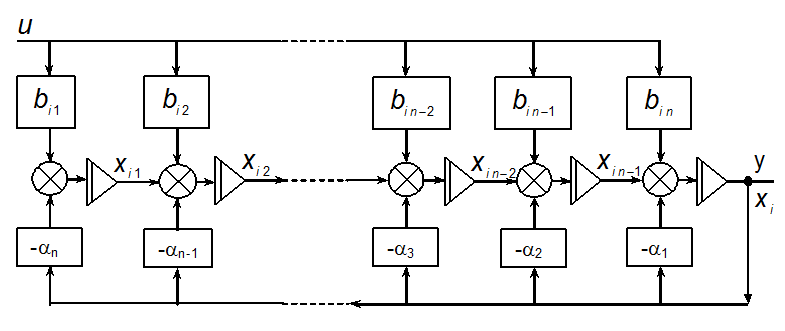
\includegraphics[scale=0.9]{images/Fig3_8}
	\caption{Схема моделирования системы в ИКП}
\end{figure}

В соответствии с этим рисунком передаточная функция системы имеет вид

\begin{multline}
	W_{u,y}(p) = \dfrac{b_{i1}p^{-n}+b_{i2}p^{-(n-1)}+\dots+b_{in-1}p^{-2}+b_{in}p^{-1}}{1+\alpha_1p^{-1}+\alpha_2p^{-2}+\dots+\alpha_np^{-n}} = \\
	\dfrac{b_{i1}+b_{i2}p+\dots+b_{in-1}p^{n-2}+b_{in}p^{n-1}}{p^n+\alpha_1p^{n-1}+\alpha_2p^{n-2}+\dots+\alpha_{n-1}p+\alpha_n}.
\end{multline}

Отметим, что статический передаточный коэффициент

\begin{equation}
	W_{u,y}(0)=\dfrac{b_{i1}}{\alpha_n}
\end{equation}

\newpage